\section{Překlad adres}
% Tady bude popsán překlad adres. Co to je, k cemu slouzi ..

Překlad síťových adres neboli NAT (Network address translation) je způsob úpravy paketů síťového provozu, kde se přepisuje zdrojová a/nebo cílová adresa a někdy také i port. Obvykle se také přepočítává kontrolní součet, který by po úpravě adres či port neodpovídal a byl by takový paket na prvním routeru zahozen.

NAT se používá především pro připojení počítačů na lokální síti do internetu, kde jsou takové počítače skryty zpravidla za jednu IP adresu. Navíc technologie překladu adres nepatrně zvyšuje bezpečnost počítačů (připojených za NATem), protože útočník nezná opravdou IP adresu \uv{zanatovaného} počítače. Nelze však NAT používat místo zabezpečení.

%------------------------------------------------------------------------------

\subsection{Cisco a NAT}
Cisco podporuje několik druhů překladu síťových adres:\cite{cisco:druhy}

\begin{itemize}
\item statický NAT
\item dynamický NAT
\item overloading
\item jakákoliv kombinace statického a dynamického NATu a overloading.
\end{itemize}

Překlad adres lze u cisca nastavit opravdu detailně, pro tuto práci je však důležitá pouze úzká podmnožina NATu. Detailní popis funkce NATu lze nalézt na webových stránkách společnosti Cisco Systems\cite{cisco:nat}.
Soukromý počítač je počítač umístěný v lokální síti. Je tedy schován za nějakou IP adresu routeru, který provádí překlad. Naopak veřejný počítač je takový počítač, který není schován za NATem (alespoň z pohledu soukromého počítače\footnote{Ale i takovýto počítač může být schován za jiným nadřazeným routerem za NAT.}).

\subsubsection{Statický NAT}
Statický překlad adres umožňuje stanovit pravidla, která říkají, na jakou adresu má být přeložen počítač s danou IP adresou. Např.:
\begin{verbatim}
ip nat inside source static 10.10.10.2 147.16.68.5
\end{verbatim} 
Tímto příkazem se bude překládat paket s adresou \verb|10.10.10.2| na adresu \verb|147.16.68.5| (za předpokladu, že paket přišel z rozhraní, které je nastavené jako soukromé, a paket míří do veřejné sítě - přes veřejné rozhraní). Statický NAT funguje i obráceným směrem. Jiné pakety (tj. od jiných počítačů) se překládat nebudou. 

Celá situace je znázorněna na obrázku \ref{fig:nat1}. U paketů od \verb|pocitac1| se bude přepisovat zdrojová IP adresa na \verb|147.16.68.5|. Zatímco pakety od \verb|pocitac2| zůstanou nezměněny.

\begin{figure}[h]
\begin{center}
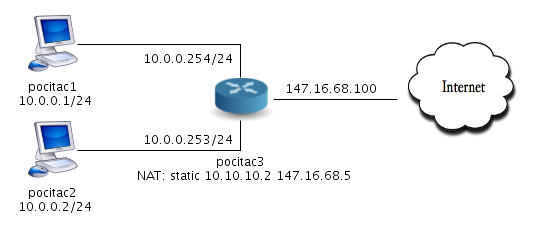
\includegraphics[width=12cm]{figures/nat1}
\caption{Statický překlad adres}
\label{fig:nat1}
\end{center}
\end{figure}

\newpage


\subsubsection{Dynamický NAT a overloading}
Dynamický překlad adres je velmi podobný statickému s tím rozdílem, že se pravidla generují dynamicky. Je pouze přiřazen pool IP adres\footnote{pool je doslova zásoba či rezerva}, ze kterého se přiřazují adresy (s portem) při překladu. Navíc lze omezit adresy sítí, které se mají překládat (příkaz \verb|access-list|).

Overloading je spíše podmnožina dynamického NATu, kde je povoleno přiřazovat jednu IP adresu více počítačům. Pakety od různých počítačů jsou pak odlišeny jiným portem.

Dynamický překlad probíhá tak, že se nejdříve zkontrolují access-listy, zda se má vůbec překládat. Když IP adresa spadá do access-listu, tak se vezme volná IP adresa (při metodě overloading může být vybrána jedna adresa vícekrát) z poolu, který je k access-listu přiřazen. Touto vybranou IP adresou počítač přepíše zdrojovou adresu příchozího paketu a vytvoří dynamický záznam do NAT tabulky. Zpětná překlad je jednodušší. Počítač vybere dynamický záznam, přepíše cílovou adresu a předá paket směrovacím pravidlům.

\paragraph{IOS příkazy}
Přidat pool adres lze příkazem:
\begin{verbatim}
ip nat pool <POOL_JMENO> <IP_START> <IP_KONEC> prefix <PREFIX>
POOL_JMENO - název poolu IP adres
IP_START - adresa, od které se budou adresy generovat
IP_KONEC - adresa, do které se budou adresy generovat
PREFIX - maska poolu v počtu jedničkových bitů
\end{verbatim} 

Přístupový list pro omezení překladu adres se přidá přes příkaz:
\begin{verbatim}
access-list <CISLO> permit <IP> <WILDCARD>
CISLO - identifikátor access-listu
IP - adresa sítě povolených IP adres
WILDCARD - maska ve tvaru wildcard (maska = broadcast - wildcard)
\end{verbatim}

Pro přiřazení poolu k access-listu se provadí pomocí příkazu:
\begin{verbatim}
ip nat inside source list <ACCESS-LIST> pool <POOL> overload?
ACCESS-LIST - identifikátor access-listu
POOL - jméno poolu
overload - nepovinná volba pro overloading
\end{verbatim} 

%------------------------------------------------------------------------------

\subsection{Návrh a implementace NATu}

\subsubsection{Návrh}
Každý počítač bude mít vlastní NAT tabulku. Ta bude složená ze seznamu \verb|NATzaznam|. Dále NAT tabulka bude potřebovat seznam soukromých rozhraní a odkaz na jedno veřejné. Bude také potřeba si držet číslo aktuálního access-listu, poolu a stav příznaku overloading. Vše ilustruje obrázek \ref{fig:nat_navrh1}.

\begin{figure}[h]
\begin{center}
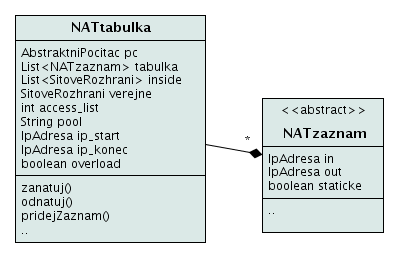
\includegraphics[width=9cm]{figures/nat_navrh1}
\caption{Návrh překladu adres č.1}
\label{fig:nat_navrh1}
\end{center}
\end{figure}

\subsubsection{Implementace}
Při implementaci NAT tabulky vyplula na povrch chyba v návrhu. Návrh počítal s tím, že může být pouze jeden pool a jeden access-list. Skutečné cisco si ale pamatuje bez problému i stovky těchto příkazů. Z tohoto důvodu jsem musel původní návrh přizpůsobit. Přidal jsem několik dalších datových struktur, které mi v pozdější fázi velmi usnadnili manipulaci s NAT tabulkou. Na obrázku \ref{fig:nat_navrh2} je znázorněn nový návrh.

\begin{figure}[b]
\begin{center}
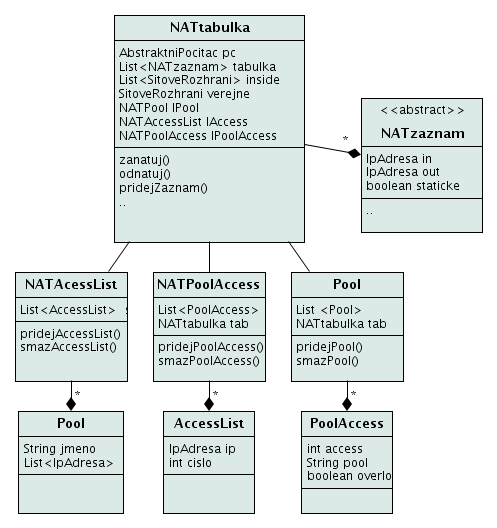
\includegraphics[width=12cm]{figures/nat_navrh2}
\caption{Návrh překladu adres č.2 - finální}
\label{fig:nat_navrh2}
\end{center}
\end{figure}

\paragraph{Postup překladu adres}
Podrobný postup překladu adres na skutečném ciscu lze nalézt na webových stránkách firmy Cisco \cite{cisco:postup}.

\subparagraph{Směr ven}
Když přijde paket do počítače, tak se nejdříve provede reverzní překlad\footnote{Reverzní překlad by v češtině nejlépe vystihoval výraz \uv{\textit{odnatování}}.}. Po té počítač dle routovací tabulky rozhodne, na které rozhraní paket odešle. Pak přichází na řadu samotný akt překladu adres. Chování NATu je řízeno několika pravidly:

\begin{itemize}
\item Když příchozí rozhraní\footnote{Rozhraní, pomocí kterého byl paket do počítače přijat.} není označeno jako soukromé\footnote{V Cisco IOSu pomocí příkazu \uv{ip nat inside}.} nebo odchozí rozhraní není označeno jako veřejné\footnote{Veřejné rozhraní je označeno příkazem \uv{ip nat outside}.}, tak se paket přepošle dál bez překladu adres.

\item Pokud lze nalézt statické pravidlo, které by odpovídalo zdrojové adrese, tak se přeloží zdrojová adresa dle tohoto pravida.

\item Když není nalezen žádný access-list, který by odpovídal zdrojové adrese, tak se paket přepošle bez překladu.

\item Když zdrojová adresa paketu spadá do access-listu, ke kterému není přiřazen žádný pool, tak se pošle zpět odesílateli \verb|Destination Host Unreacheble|.

\item Když v IP poolu, který je přiřazen k odpovídajícímu access-listu, dojdou volné IP adresy, tak se pošle zpět odesílateli \verb|Destination Host Unreacheble|.

\item V ostatních případech se provede překlad adres:
    \begin{enumerate}
    \item Zkusí se nalézt odpovídající dynamické pravidlo. V případě nenalezení viz následující bod.
    \item Vygeneruje se nová IP adresa z poolu a vloží se takto vytvořený záznam do NAT tabulky.
    \end{enumerate}
\end{itemize}

Vše je lépe znázorněno na vývojovém diagramu \ref{fig:nat_decision}.

\begin{figure}[b]
\begin{center}
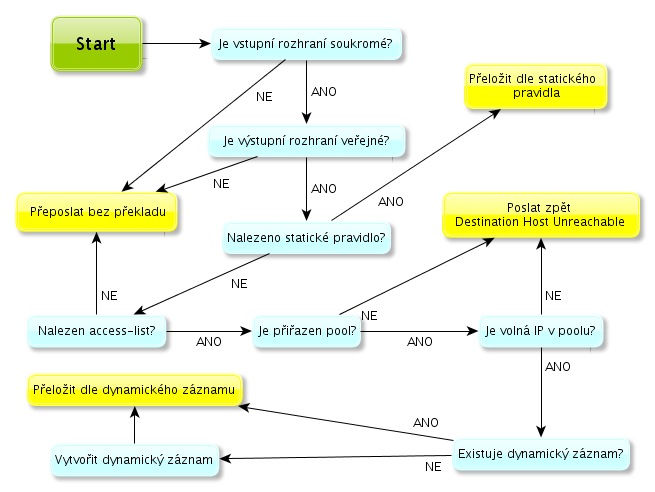
\includegraphics[width=16cm]{figures/nat_decision}
\caption{Vývojový diagram překladu adres}
\label{fig:nat_decision}
\end{center}
\end{figure}

% routovani
% zanatovava se kdyz je prichozi soukrome, kdyz odchozi je verejne
% musit patrit do access-listu (kdyz nepatri, tak jen preposlat bez odnatovani)
% k nemu musi byt prirazen pool (kdyz neni tak se posila zpet DHU)
% kdyz neni volna IP (už došli), tak se posle zpet DHU
% IP je v a-listech && je volná IP tak se natuje:
%     pokud je stat. prav. tak se zanatuje
%     pokud je dyn. prav. tak se zanatuje
%     kdyz nic, tak se vygeneruje novy dyn. zaznam a prida se do tabulky
%     prelozi je zdrojova a odesle do vnejsi site



\subparagraph{Směr dovnitř - reverzní překlad}

Reverzní překlad je mnohem jednodušší záležitost. Příchozí paket čekají tyto pravidla:
\begin{enumerate}
  \item Nejdříve se zkontroluje, zda paket přišel přes veřejné rozhraní. Když je vstupní rozhraní jiné než neřejné, tak se reverzní překlad neprovede.

  \item Pak se prohledají statická pravidla, zda nějaké odpovídá (včetně portu) cílové adrese paketu. Pokud odpovídá, tak se provede reverzní překlad.

  \item Když se nenajde ani žádný dynamický záznam, tak se cílová adresa paketu překládat nebude a paket zůstane beze změny.
\end{enumerate}


\subsubsection*{}
Z obou směrů překladu vyplývá, že statická pravidla mají přednost před dynamickými záznamy. Při testování NATu na školních ciscách jsem zjistil, že cisca zapomínají všechny dynamické záznamy starší cca 10 vteřin. Tato vlastnost byla dodatečně implementována i do této aplikace. Více informací o konfiguraci statického a dynamického NATu zároveň je na stránkách Cisco Systems \cite{cisco:snat_dnat}.




% odnatovava se kdyz je nastaveno verejne rozhr. a kdyz to taky z nej prislo
% juk do tabulky - staticke, pak dyn.
% pak smerovani
% odeslani do vnitrni site





